\documentclass{beamer}
%\usetheme{Rochester}
\usetheme{Copenhagen}
%\usetheme{Madrid}
\usepackage{graphicx}

\title{The Go Programming Language}
\subtitle{http://www.golang.org \\ CS 239: Parallel Programming Languages}
\author{Raghu Prabhakar \\ Rohit Kumar}
\date{June 2, 2011}
\begin{document}

\begin{frame}
\begin{center}

\includegraphics[width=1in]{gopher.png}
\end{center}
\titlepage
\end{frame}

\begin{frame} {About Go}
\begin{itemize}
  \item Developed by Google. Released in 2009.
  \item Rob Pike, Ken Thompson, Robert Griesemer
  \item Compiled, garbage collected, concurrent, statically typed,
    imperative. 
  \item UTF-8 Support
  \item Borrows from CSP, Occam and Erlang
  \item Compilers: 6g, 8g, gcc 
\end{itemize}
\end{frame}

\begin{frame}{Concurrency}
  \begin{itemize}
    \item Go-routines
    \item Channels
    \item WaitGroup
  \end{itemize}
\end{frame}

\begin{frame} [fragile]
\frametitle{Go-routines}
\begin{itemize}
  \item Go-routines $\approx$ \verb=async=
\end{itemize}
\begin{center}
\begin{verbatim}
                go mapblock(start, end)
\end{verbatim}
\end{center}
\end{frame}

\begin{frame} [fragile]
\frametitle{Channels}
\begin{itemize}
\item Means to send and receive messages
\item Channels are typed
\end{itemize}
\begin{verbatim}
        var ch = make(chan int) 
        ch <- 42 // send 
        var i = <- ch // receive        
\end{verbatim}
\begin{center}
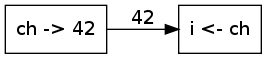
\includegraphics[width=2in]{channel.png}
\end{center}
\end{frame}

\begin{frame}{Channels}

\begin{itemize}
\item Buffered and unbuffered
\item Unbuffered -- block on send and receive
\item Buffered  -- block on send only if buffer is full. Block on receive.

\end{itemize}
\end{frame}

\begin{frame}[fragile]
\frametitle{Channels}
\begin{itemize}
\item Channels can be used to model \verb=finish= like behavior
\end{itemize}
\begin{verbatim}
        var ch = make(chan bool)
        for i:=0; i < n ; i++ {
                go func() { 
                        // do something
                        ch <- true
                } ()
        }
\end{verbatim}
\pause
\begin{verbatim}
        // drain the channel
        for i:=0; i < n; i++ {
                <- ch
        }
        close(ch)
        
\end{verbatim}
\end{frame}

\begin{frame}{Select}
\end{frame}

\begin{frame} {WaitGroup}

\end{frame}

\begin{frame} {Map Reduce}
\end{frame}

\begin{frame} {Parallel Prefix Sum}
\end{frame}

\end{document}
